\documentclass{beamer}

\usepackage{comment}
\usepackage{color}
\usepackage{listings}
\usepackage{verbatim}
\usepackage{multicol}
\usepackage{booktabs}
\definecolor{green}{RGB}{0,128,0}

\def\EQ#1\EN{\begin{equation*}#1\end{equation*}}
\def\BA#1\EA{\begin{align*}#1\end{align*}}
\def\BS#1\ES{\begin{split*}#1\end{split*}}
\newcommand{\bc}{\begin{center}}
\newcommand{\ec}{\end{center}}
\newcommand{\eq}{\ =\ }
\newcommand{\degc}{$^\circ$C}

\def\p{\partial}
\def\qbs{\boldsymbol{q}}
\def\Dbs{\boldsymbol{D}}
\def\A{\mathcal A}
\def\gC{\mathcal C}
\def\gD{\mathcal D}
\def\gL{\mathcal L}
\def\M{\mathcal M}
\def\P{\mathcal P}
\def\Q{\mathcal Q}
\def\gR{\mathcal R}
\def\gS{\mathcal S}
\def\X{\mathcal X}
\def\bnabla{\boldsymbol{\nabla}}
\def\bnu{\boldsymbol{\nu}}
\renewcommand{\a}{{\alpha}}
%\renewcommand{\a}{{}}
\newcommand{\s}{{\sigma}}
\newcommand{\bq}{\boldsymbol{q}}
\newcommand{\bz}{\boldsymbol{z}}
\def\bPsi{\boldsymbol{\Psi}}

\def\Li{\textit{L}}
\def\Fb{\textbf{f}}
\def\Jb{\textbf{J}}
\def\cb{\textbf{c}}

\def\Dt{\Delta t}
\def\tpdt{{t + \Delta t}}
\def\bpsi{\boldsymbol{\psi}}
\def\dbpsi{\delta \boldsymbol{\psi}}
\def\bc{\textbf{c}}
\def\dbc{\delta \textbf{c}}
\def\arrows{\rightleftharpoons}

\newcommand{\bGamma}{\boldsymbol{\Gamma}}
\newcommand{\bOmega}{\boldsymbol{\Omega}}
%\newcommand{\bPsi}{\boldsymbol{\Psi}}
%\newcommand{\bpsi}{\boldsymbol{\psi}}
\newcommand{\bO}{\boldsymbol{O}}
%\newcommand{\bnu}{\boldsymbol{\nu}}
\newcommand{\bdS}{\boldsymbol{dS}}
\newcommand{\bg}{\boldsymbol{g}}
\newcommand{\bk}{\boldsymbol{k}}
%\newcommand{\bq}{\boldsymbol{q}}
\newcommand{\br}{\boldsymbol{r}}
\newcommand{\bR}{\boldsymbol{R}}
\newcommand{\bS}{\boldsymbol{S}}
\newcommand{\bu}{\boldsymbol{u}}
\newcommand{\bv}{\boldsymbol{v}}
%\newcommand{\bz}{\boldsymbol{z}}
\newcommand{\pressure}{P}

\def\water{H$_2$O}
\def\calcium{Ca$^{2+}$}
\def\copper{Cu$^{2+}$}
\def\magnesium{Mg$^{2+}$}
\def\sodium{Na$^+$}
\def\potassium{K$^+$}
\def\uranium{UO$_2^{2+}$}
\def\hion{H$^+$}
\def\hydroxide{0H$^-$}
\def\bicarbonate{HCO$_3^-$}
\def\carbonate{CO$_3^{2-}$}
\def\cotwo{CO$_2$(aq)}
\def\chloride{Cl$^-$}
\def\fluoride{F$^-$}
\def\phosphoricacid{HPO$_4^{2-}$}
\def\nitrate{NO$_3^-$}
\def\sulfate{SO$_4^{2-}$}
\def\souotwooh{$>$SOUO$_2$OH}
\def\sohuotwocothree{$>$SOHUO$_2$CO$_3$}
\def\soh{$>$SOH}

\newcommand\gehcomment[1]{{{\color{orange} #1}}}
\newcommand\add[1]{{{\color{blue} #1}}}
\newcommand\remove[1]{\sout{{\color{red} #1}}}
\newcommand\codecomment[1]{{{\color{green} #1}}}
\newcommand\redcomment[1]{{{\color{red} #1}}}
\newcommand\bluecomment[1]{{{\color{blue} #1}}}
\newcommand\greencomment[1]{{{\color{green} #1}}}
\newcommand\magentacomment[1]{{{\color{magenta} #1}}}

\begin{comment}
\tiny
\scriptsize
\footnotesize
\small
\normalsize
\large
\Large
\LARGE
\huge
\Huge
\end{comment}

\begin{document}
\title{3D Regional Flow and Transport \ldots in a Nutshell}
\author{Glenn Hammond}
\date{\today}

%\frame{\titlepage}

%-----------------------------------------------------------------------------
\section{Description of 3D Regional Flow and Transport Model}

\subsection{3D Regional Flow and Transport Model}

\frame{\frametitle{Description of 3D Regional Flow and Transport Scenario}
The ``3D Regional Flow and Transport Scenario'' simulates groundwater flow and solute transport within a large kilometer-scale domain:
\begin{itemize}
  \item Problem domain: $5000 \times 2500 \times 100$ m$^3$ ($x \times y \times z$)
  \item Grid resolution $50 \times 49.02 \times 5$ m$^3$ ($100 \times$ 51 $\times$ 20 cells)
  \item Maximum time step size: 0.1 y (for CFL $<= 1$)
  \item Total simulation time: 10 y
\end{itemize}

}

%-----------------------------------------------------------------------------
\frame{\frametitle{3D Regional Flow and Transport Scenario Schematic}
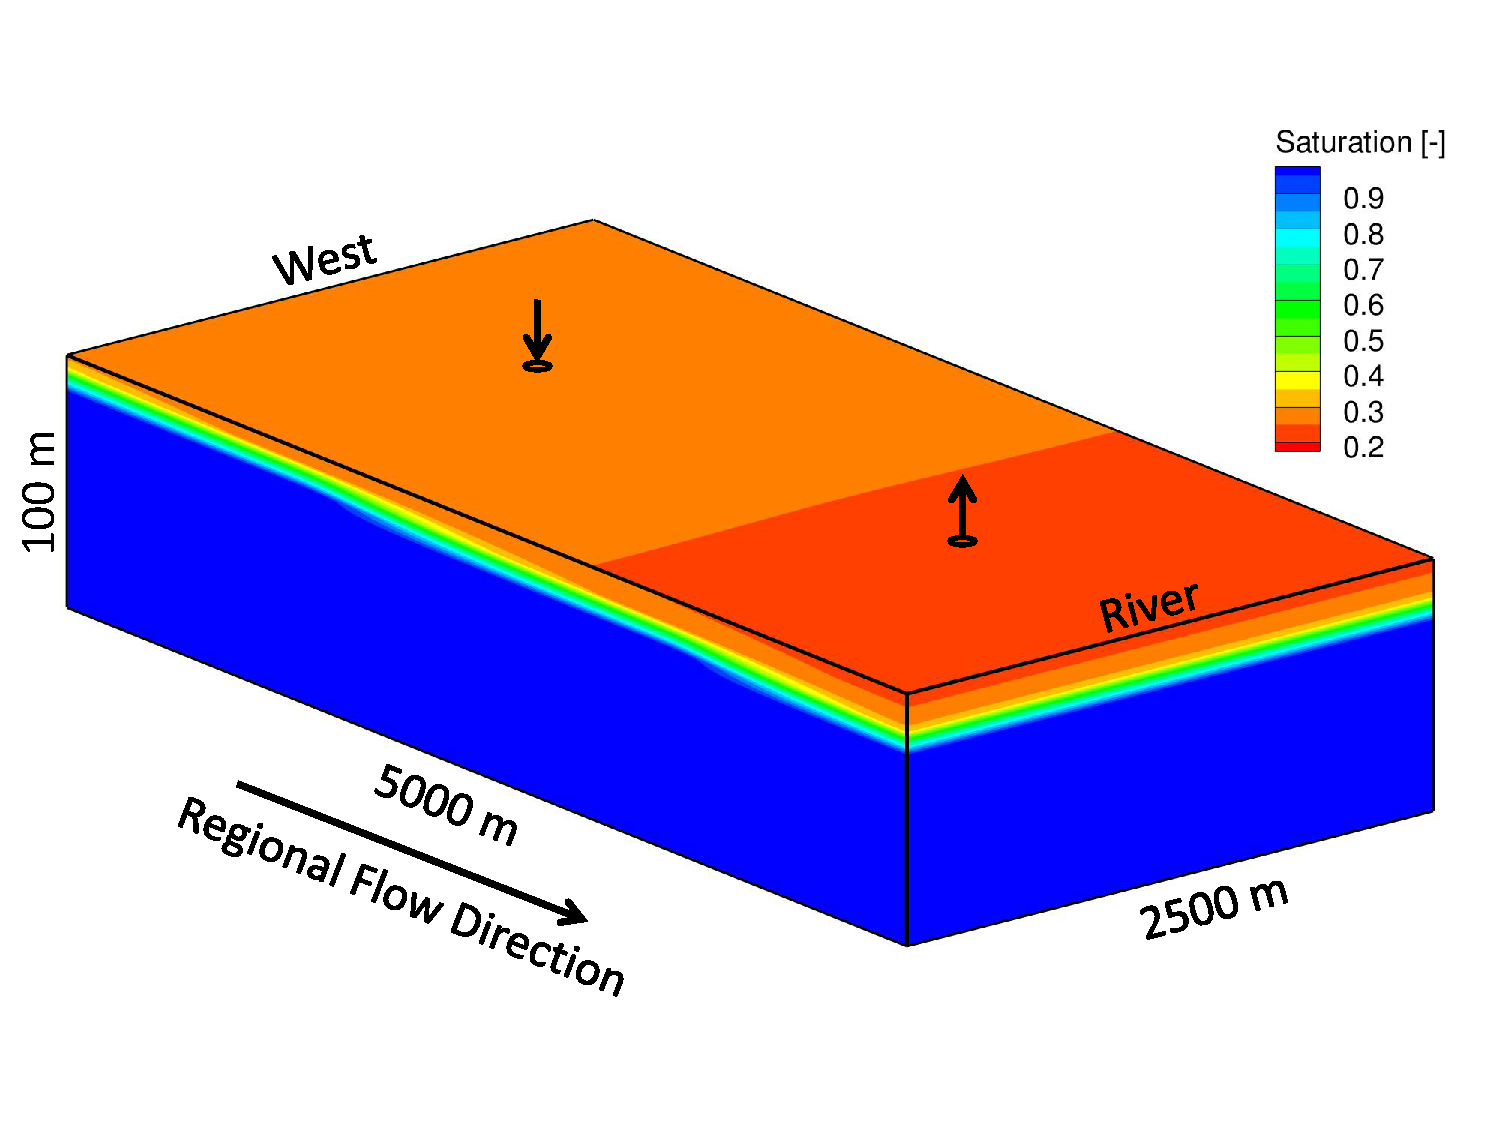
\includegraphics[width=\linewidth]{./regional_doublet_fig}
}

%-----------------------------------------------------------------------------
\subsection{Flow Governing Equations}

\frame{\frametitle{Governing Flow Equations}

{\bf Continuity Equation:}
\EQ
\frac{\p}{\p t} \big(\varphi s \rho\big) + \bnabla\cdot\rho\bq \eq Q
\EN


{\bf Darcy's Law:}
\EQ
\bq \eq -\frac{\bk k_r}{\mu} \bnabla\big(\pressure-\rho g z\big)
\EN

\normalsize

\begin{columns}[c]
\column{0.5\linewidth}
\begin{itemize}
\item $\varphi \eq $ porosity
\item $s \eq $ saturation
\item $\rho \eq $ water density
\item $\bk \eq $ intrinsic permeability tensor
\item $k_r \eq $ relative permeability
\end{itemize}
\column{0.5\linewidth}
\begin{itemize}
\item $\mu \eq $ viscosity
\item $\pressure \eq $ water pressure
\item $g \eq $ gravity
\item $z \eq $ distance in direction of gravity
\item $Q \eq $ source/sink
\end{itemize}
\end{columns}

}

%-----------------------------------------------------------------------------
\frame{\frametitle{Constitutive Relations
%\dblline
}
\begin{itemize}
\item Capillary Pressure Relations
\begin{itemize}
\item van Genuchten
\begin{itemize}
\item Effective Saturation:
\EQ\label{seff}
s_e \eq \left[1+\left( \alpha |P_c| \right)^n \right]^{-m}\nonumber
\EN
\item Saturation:
\EQ
s \eq s_e (1-s_r)+s_r
\EN
\item Relative Permeability (Mualem)
\EQ\label{krl}
k_r \eq \sqrt{s_e} \left\{1-\left[1-s_e^{1/m} \right]^m \right\}^2\nonumber
\EN

\end{itemize}
\end{itemize}
\end{itemize}

\bigskip
\footnotesize
\begin{columns}[c]
\column{0.6\linewidth}
\begin{itemize}
\item $s \eq $ saturation
\item $s_e \eq $effective saturation
\item $s_r \eq $ residual saturation
\item $P_c \eq $ capillary pressure $\eq P_\text{atm} - \pressure$
\end{itemize}
\column{0.4\linewidth}
\begin{itemize}
\item $\alpha \eq $ inverse of air entry pressure [Pa$^{-1}$]
\item $n \eq $ van Genuchten $n$
\item $m \eq 1 - 1/n$
\end{itemize}
\end{columns}

}

%-----------------------------------------------------------------------------
\frame{
\frametitle{Constitutive Relations [Cont.]
%\dblline
}

\begin{itemize}
\item[]
\begin{itemize}
\item Brooks-Corey
\begin{itemize}
\item Effective Saturation:
\EQ\label{seffbc}
s_e \eq \left( \alpha |P_c| \right)^{-\lambda}\nonumber
\EN
\item Saturation:
\EQ
s \eq s_e (1-s_r)+s_r
\EN
\item Relative permeability (Burdine)
\BA
k_r &\eq \left(s_e \right)^{(2+3\lambda)/\lambda}\nonumber\\
&\eq \left( \alpha |P_c| \right)^{-(2+3\lambda)}\nonumber \label{krlbc}
\EA
\end{itemize}
\end{itemize}
\end{itemize}

\bigskip
\footnotesize
\begin{columns}[c]
\column{0.6\linewidth}
\begin{itemize}
\item $\alpha \eq $ inverse of air entry pressure [Pa$^{-1}$]
\item $\lambda \eq $Brooks Corey function parameter $\lambda$
\end{itemize}
\column{0.4\linewidth}
\begin{itemize}
\item[]
\item[]
\end{itemize}
\end{columns}
}

%-----------------------------------------------------------------------------
\frame{\frametitle{Flow Boundary Conditions}

\begin{itemize}
\item Dirichlet (e.g. specified pressure)
\item Neumann (e.g. specified flux)
\end{itemize}

\begin{itemize}
\item No Flow
\item Recharge
\item Hydrostatic
\item Seepage Face
\end{itemize}

}

%-----------------------------------------------------------------------------
\frame{\frametitle{Flow Boundary Conditions Schematic}
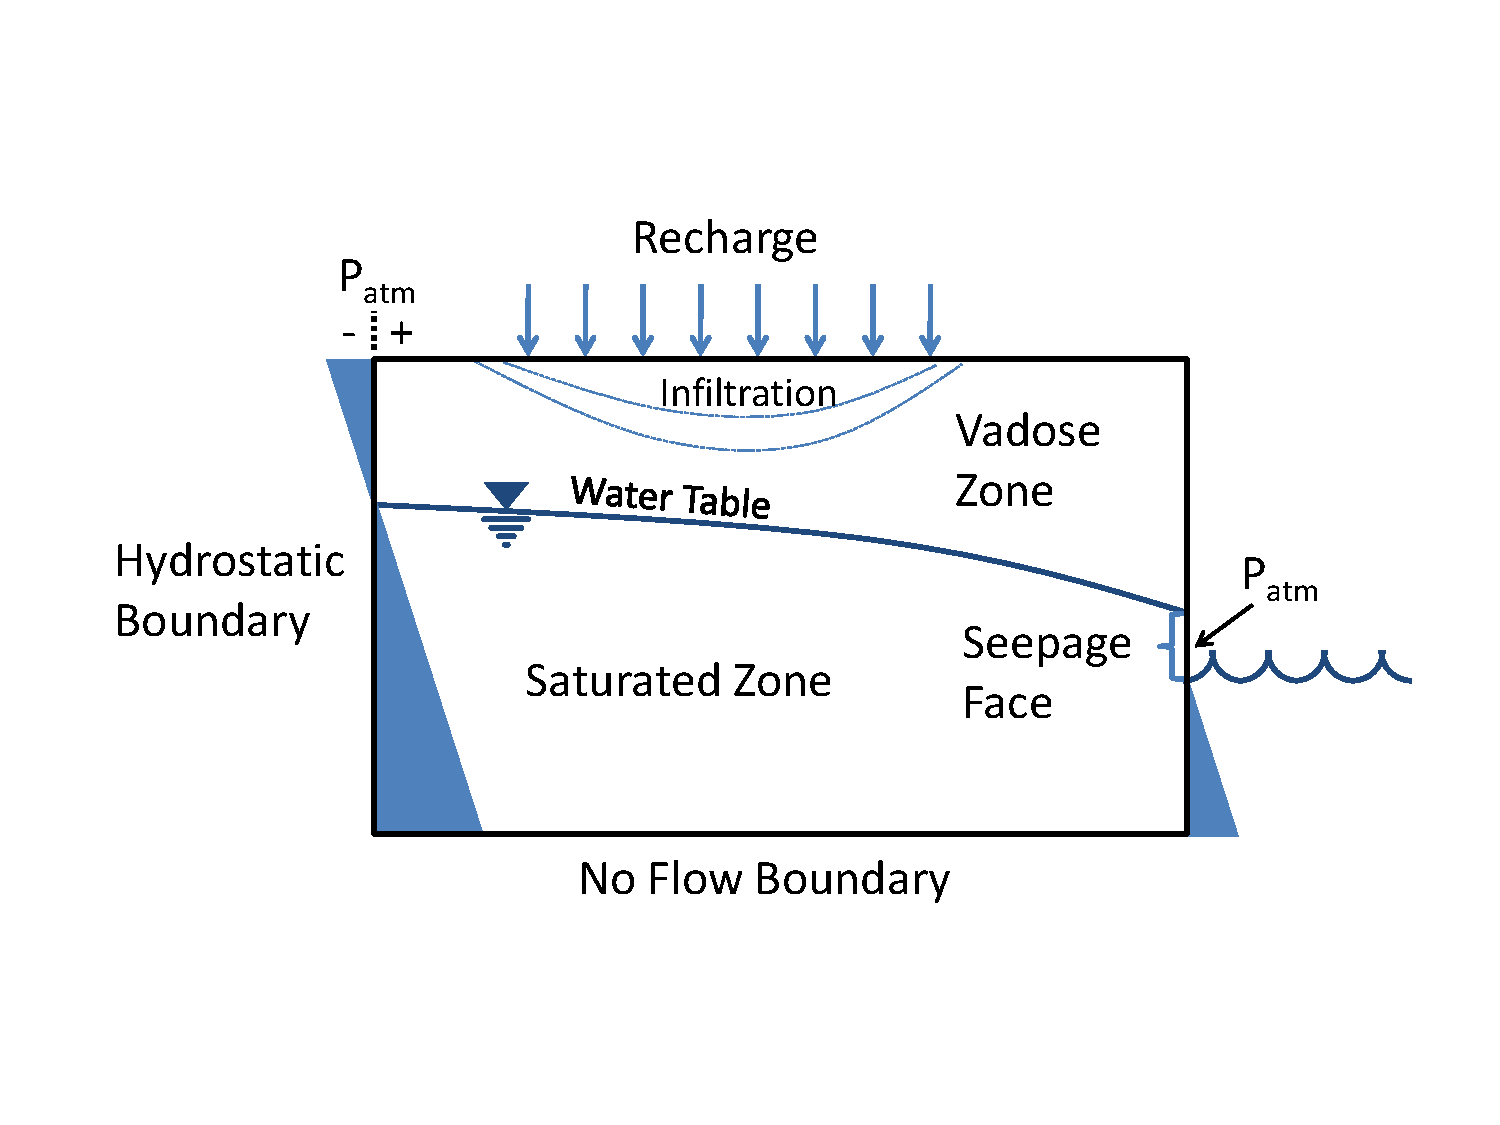
\includegraphics[width=\linewidth]{./flow_bcs}
}

\frame{\frametitle{Flow Boundary Conditions}

\large
\EQ
\bq \eq -\frac{kk_r}{\mu} \left(\frac{\pressure_\text{cell}-\pressure_\text{boundary}-\rho g \bz}{\Delta l}\right)
\EN

\bigskip
\small
\begin{itemize}
\item $\bq$ units: $\left[\frac{l^3_\text{water}}{l^2_\text{bulk} \cdot t}\right]$ where $l \eq$ length and $t \eq$ time
\item[]
\item No flow (Neumann) : $\bq = 0$ or even better, no flux calculation at all
\item Recharge (Neumann) : $\bq = \bq_0$
\item Hydrostatic (Dirichlet): $\pressure_\text{boundary} \eq f\left(\pressure_\text{datum},x,y,z,\rho\left(P,T\right)\right)$
\item Seepage Face (Dirichlet) : $\pressure_\text{boundary} \eq max\left(\text{Hydrostatic},\pressure_\text{atm}\right)$
\end{itemize}

}

%-----------------------------------------------------------------------------
\frame{\frametitle{Richards Equation - Averaging Schemes}

\Large
\EQ
\bq \eq -\frac{\bk k_r}{\mu} \bnabla\big(\pressure-\rho g z\big)
\EN

%\normalsize
\begin{itemize}
\item $\bk$: harmonic
\item $k_r$: upwind
\item $\mu$: upwind
\item $\rho$: arithmetic

\end{itemize}
}

%-----------------------------------------------------------------------------
\subsection{Transport Governing Equations}

\frame{\frametitle{Governing Transport Equations}

\Large

\EQ\label{trans}
\frac{\p}{\p t} \left(\varphi s \Psi_j\right) + \bnabla\cdot\bOmega_j \eq S_j
\EN

\EQ\label{flux}
\bOmega_j \eq \big(\bq - \varphi s \Dbs\bnabla\big) \Psi_j
\EN

%\bigskip
%\normalsize
\footnotesize
\begin{align*}
\varphi &\eq \text{porosity}; \quad
s \eq \text{liquid saturation}\\
\Psi_j &\eq \text{solute concentration for aqueous species } j\\
S_j &\eq \text{source/sink term for aqueous species } j\\
\bOmega &\eq \text{solute flux}; \quad
\bq \eq \text{Darcy velocity} \\
\Dbs &\eq \text{hydrodynamic dispersion} \eq\gD^\ast + \alpha_L|\bnu|\\
\gD^\ast &\eq \text{species {\color{red} independent} coefficient of diffusion}\\
\alpha_L &\eq \text{longitudinal dispersity}\\
\bnu &\eq \text{pore water velocity} \eq \bq/\varphi
\end{align*}

}

%-----------------------------------------------------------------------------
\frame{\frametitle{Transport Boundary Conditions}

\begin{itemize}
\item Dirichlet (e.g. specified concentration)
\item Neumann (e.g. specified mass flux)
\item Zero Gradient (e.g. outflow boundary)
\end{itemize}


}

%-----------------------------------------------------------------------------
\frame{\frametitle{Transport - Averaging Schemes}
\Large
\EQ\label{flux}
\bOmega_j \eq \big(\bq - \varphi s \Dbs\bnabla\big) \Psi_j
\EN

\bigskip
%\normalsize
\begin{itemize}
\item $s$: arithmetic
\item $\varphi$: arithmetic
\end{itemize}
}

%-----------------------------------------------------------------------------
\section{Description of Input Deck}

\subsection{SIMULATION}
\begin{frame}[fragile,containsverbatim]\frametitle{SIMULATION}

\begin{itemize}
  \item Single-phase variably saturated flow
  \item Conservative solute transport
\end{itemize}

\begin{semiverbatim}
SIMULATION
  SIMULATION_TYPE SUBSURFACE
  PROCESS_MODELS
    SUBSURFACE_FLOW flow
      MODE RICHARDS
    /
    SUBSURFACE_TRANSPORT transport
      GLOBAL_IMPLICIT
    /
  /
END

SUBSURFACE
  ...
END_SUBSURFACE
\end{semiverbatim}

\end{frame}

%-----------------------------------------------------------------------------
\begin{frame}[fragile,containsverbatim]\frametitle{GRID}

\begin{itemize}
  \item Problem domain: $5000 \times 2500 \times 100$ m (x $\times$ y $\times$ z)
  \item Grid resolution $50 \times 49.02 \times 5$ m
\end{itemize}

\begin{semiverbatim}
GRID
  TYPE structured
  NXYZ 100 51 20
  BOUNDS
    0.d0 0.d0 0.d0
    5000.d0 2500.d0 100.d0
  /
END
\end{semiverbatim}

\end{frame}

%-----------------------------------------------------------------------------
\subsection{REGION}

\begin{frame}[fragile,containsverbatim,allowframebreaks]\frametitle{REGION}

\begin{itemize}
  \item Delineate regions in the 3D domain for:
  \begin{itemize}
    \item entire domain
    \item west boundary face
    \item east boundary face
    \item top boundary face
    \item well screens
  \end{itemize}
\end{itemize}

\begin{semiverbatim}
REGION all
  COORDINATES
    0.d0 0.d0 0.d0
    5000.d0 2500.d0 100.d0
  /
END

\newpage
REGION layer2        \bluecomment{! layer of domain}
  COORDINATES
    0.d0 0.d0 30.d0
    5000.d0 2500.d0 50.d0
  /
END

REGION Top           \bluecomment{! top surface}
  COORDINATES
    0.d0 0.d0 100.d0
    5000.d0 2500.d0 100.d0
  /
  FACE TOP
END

\newpage
REGION Extraction_well
  COORDINATES             \bluecomment{! vertical line}
    3750.d0 1250.d0 20.d0
    3750.d0 1250.d0 55.d0
  /
END

REGION Obs_pt_center      \bluecomment{! point}
  \magentacomment{COORDINATE} 2500.d0 1250.d0 60.d0
END

\end{semiverbatim}

\end{frame}


%-----------------------------------------------------------------------------
\subsection{MATERIAL\_PROPERTY}

\begin{frame}[fragile,containsverbatim]\frametitle{MATERIAL\_PROPERTY}

\begin{itemize}
  \item Anisotropic permeability
\end{itemize}

\begin{semiverbatim}
MATERIAL_PROPERTY soil3
  ID 3
  POROSITY 0.25d0
  TORTUOSITY 0.5d0
  CHARACTERISTIC_CURVES cc1
  PERMEABILITY        \bluecomment{! diagonal permeability tensor}
    PERM_X 5.d-11     \bluecomment{!   x component}
    PERM_Y 5.d-11     \bluecomment{!   y component}
    PERM_Z 5.d-12     \bluecomment{!   z component}
  /
END
\end{semiverbatim}

\end{frame}

%-----------------------------------------------------------------------------
\subsection{CHARACTERISTIC\_CURVES}

\begin{frame}[fragile]\frametitle{CHARACTERISTIC\_CURVES}

\begin{itemize}
\item van Genuchten saturation function
\item Mualem relative permeability
\end{itemize}

\begin{semiverbatim}
CHARACTERISTIC_CURVES cc1
  SATURATION_FUNCTION VAN_GENUCHTEN
    ALPHA  1.d-4
    M 0.5d0
    LIQUID_RESIDUAL_SATURATION 0.1d0
    MAX_CAPILLARY_PRESSURE 1.d8
  /
  PERMEABILITY_FUNCTION MUALEM_VG_LIQ
    M 0.5d0
    LIQUID_RESIDUAL_SATURATION 0.1d0
  /
END
\end{semiverbatim}

\end{frame}

%-----------------------------------------------------------------------------
\subsection{FLUID\_PROPERTY}

\begin{frame}[fragile,containsverbatim]\frametitle{FLUID\_PROPERTY}

\begin{itemize}
  \item Assign a molecular diffusion coefficient of $10^{-9}$ m$^2$/s to all aqueous species
\end{itemize}

\begin{semiverbatim}

FLUID_PROPERTY
  DIFFUSION_COEFFICIENT 1.d-9   \bluecomment{! [m^2/s]}
END
\end{semiverbatim}

\end{frame}

%-----------------------------------------------------------------------------
\subsection{CHEMISTRY}

\begin{frame}[fragile,allowframebreaks]\frametitle{CHEMISTRY}

\begin{itemize}
\item Two tracers
\item Database is not needed!
\end{itemize}

\begin{semiverbatim}
CHEMISTRY
  PRIMARY_SPECIES
    Tracer
    Tracer2
  /
END
\end{semiverbatim}

\end{frame}

%-----------------------------------------------------------------------------
\subsection{FLOW\_CONDITION}

\begin{frame}[fragile,allowframebreaks]\frametitle{FLOW\_CONDITION}

\begin{semiverbatim}

FLOW_CONDITION initial
  TYPE
    PRESSURE HYDROSTATIC  \bluecomment{! hydrostatic condition}
  /
  DATUM 0.d0 0.d0 90.d0   \bluecomment{! point in space}
  GRADIENT
    PRESSURE -0.002 0. 0. \bluecomment{! gradient for pressure \redcomment{[m/m]}}
  /                       \bluecomment{!   unless \redcomment{dz} specified \redcomment{[Pa/m]}}
  PRESSURE 101325.d0      \bluecomment{! pressure at datum}
END

\newpage

FLOW_CONDITION river
  TYPE
    PRESSURE SEEPAGE     \bluecomment{! seepage face condition}
  /
  INTERPOLATION LINEAR   \bluecomment{! dataset time interpolation}
  CYCLIC                 \bluecomment{! cycle dataset}
  DATUM FILE river_stage.txt  \bluecomment{! read transient datum}
  PRESSURE 101325.d0          \bluecomment{!    dataset from file}
END

\newpage

\bluecomment{! Contents of river_stage.txt:}
\bluecomment{!   Note: assumes SI units}

\bluecomment{: time x y z}
0.d0 5000.d0 0.d0 80.d0          \bluecomment{! 0 yr}
7884000.d0 5000.d0 0.d0 77.d0    \bluecomment{! 0.25 yr}
15768000.d0 5000.d0 0.d0 79.d0   \bluecomment{! 0.5 yr}
23652000.d0 5000.d0 0.d0 79.d0   \bluecomment{! 0.75 yr}
31536000.d0 5000.d0 0.d0 80.d0   \bluecomment{! 1 yr}

\newpage
FLOW_CONDITION recharge
  TYPE
    FLUX NEUMANN
  /
  FLUX LIST
    TIME_UNITS yr
    DATA_UNITS cm/yr
    0.d0 25.d0
    1.d0 23.d0
    ...
    4.d0 24.d0
    5.d0 29.d0
  /
END

\newpage
FLOW_CONDITION injection
  TYPE                           \bluecomment{! volumetric flow}
    RATE SCALED_VOLUMETRIC_RATE  \bluecomment{!   rate scaled by}
  /                              \bluecomment{!   f(permeability)}
  RATE 1.d5 m^3/day  \bluecomment{! flow rate 10,000 [m^3/day]}
END

FLOW_CONDITION extraction
  TYPE
    RATE SCALED_VOLUMETRIC_RATE
  /
  RATE -1.d5 m^3/day  \bluecomment{! flow rate -10,000 [m^3/day]}
END                   \bluecomment{! negative rate = extraction}

\end{semiverbatim}
\end{frame}

%-----------------------------------------------------------------------------
\subsection{TRANSPORT\_CONDITION / CONSTRAINT}

\begin{frame}[fragile,allowframebreaks]\frametitle{TRANSPORT\_CONDITION / CONSTRAINT}

\begin{itemize}
  \item Set up three transport conditions and constraints for tracers
  \item Constraints embedded within transport conditions
  \begin{itemize}
    \item Embedded constraints may not be transient
  \end{itemize}
\end{itemize}

\newpage
{
\begin{semiverbatim}

TRANSPORT_CONDITION initial      \bluecomment{! previous approach}
  TYPE DIRICHLET_ZERO_GRADIENT
  \magentacomment{CONSTRAINT_LIST       \bluecomment{! list of constraints}
    0.d0 initial  }
  /
END

TRANSPORT_CONDITION initial      \bluecomment{! embedded approach}
  TYPE DIRICHLET_ZERO_GRADIENT
  \magentacomment{CONSTRAINT initial
    CONCENTRATIONS      \bluecomment{! single constraint @ time 0.}
      Tracer  1.d-10 T  \bluecomment{! background concentration set}
      Tracer2 1.d-10 T  \bluecomment{!   to a small value, not zero}
    /}
  /
END
\end{semiverbatim}
}

\newpage
{\small
\begin{semiverbatim}
TRANSPORT_CONDITION west
  TYPE DIRICHLET_ZERO_GRADIENT
  CONSTRAINT west
    CONCENTRATIONS
      Tracer  1.d-10 T
      Tracer2 1.d0   T
    /
  /
END

TRANSPORT_CONDITION injection
  TYPE DIRICHLET_ZERO_GRADIENT
  CONSTRAINT injection
    CONCENTRATIONS
      Tracer  1.d0   T
      Tracer2 1.d-10 T
    /
  /
END
\end{semiverbatim}
}

\end{frame}

%-----------------------------------------------------------------------------
\subsection{STRATA}

\begin{frame}[fragile]\frametitle{STRATA}

\begin{itemize}
\item Couple material types with regions
\end{itemize}

\begin{semiverbatim}
STRATA
  REGION layer1
  MATERIAL soil1
END

STRATA
  REGION layer2
  MATERIAL soil2
END

\ldots

STRATA
  REGION layer4
  MATERIAL soil4
END
\end{semiverbatim}

\end{frame}


%-----------------------------------------------------------------------------
\subsection{OBSERVATION}

\begin{frame}[fragile]\frametitle{OBSERVATION}

\begin{itemize}
\item Couple observation points with regions in model
\end{itemize}

\begin{semiverbatim}
OBSERVATION  \bluecomment{! observation point assigned region name}
  REGION Obs_pt_center  \bluecomment{! region name}
  AT_CELL_CENTER        \bluecomment{! do not interpolate}
  VELOCITY              \bluecomment{! include velocity}
END

OBSERVATION
  REGION Obs_pt_west
  AT_CELL_CENTER
  VELOCITY
END

\dots
\end{semiverbatim}

\end{frame}

%-----------------------------------------------------------------------------
\subsection{NEWTON\_SOLVER}

\begin{frame}[fragile]\frametitle{NEWTON\_SOLVER}

\begin{itemize}
  \item Set converged if maximum pressure change within all cells is less than 1 Pa.
\end{itemize}

\begin{semiverbatim}

NEWTON_SOLVER FLOW
  ITOL_UPDATE 1.d0   \bluecomment{! infinity norm of update vector}
END
\end{semiverbatim}

\end{frame}

%-----------------------------------------------------------------------------
\subsection{INITIAL\_CONDITION}

\begin{frame}[fragile]\frametitle{INITIAL\_CONDITION}

\begin{itemize}
\item Couple the greencomment{initial} flow and transport conditions with region \greencomment{all} for the initial condition
\end{itemize}

\begin{semiverbatim}

INITIAL_CONDITION
  FLOW_CONDITION initial
  TRANSPORT_CONDITION initial
  REGION all
END

\end{semiverbatim}

\end{frame}

%-----------------------------------------------------------------------------
\subsection{BOUNDARY\_CONDITION}

\begin{frame}[fragile,allowframebreaks]\frametitle{BOUNDARY\_CONDITION}

\small
\begin{semiverbatim}
BOUNDARY_CONDITION west
  FLOW_CONDITION initial
  TRANSPORT_CONDITION west
  REGION west
END

BOUNDARY_CONDITION east
  FLOW_CONDITION river
  TRANSPORT_CONDITION initial
  REGION east
END

BOUNDARY_CONDITION top
  FLOW_CONDITION recharge
  TRANSPORT_CONDITION initial
  REGION top
END
\end{semiverbatim}

\end{frame}

%-----------------------------------------------------------------------------
\subsection{SOURCE\_SINK (CONDITION)}

\begin{frame}[fragile,allowframebreaks]\frametitle{SOURCE\_SINK}

\begin{semiverbatim}
SOURCE_SINK injection_well   \bluecomment{! source/sink name (optional)}
  FLOW_CONDITION injection       \bluecomment{! flow condition name}
  TRANSPORT_CONDITION injection  \bluecomment{! tran. condition name}
  REGION injection_well        \bluecomment{! location of source/sink}
END

SOURCE_SINK extraction_well
  FLOW_CONDITION extraction
  TRANSPORT_CONDITION initial
  REGION extraction_well
END
\end{semiverbatim}

\end{frame}

%-----------------------------------------------------------------------------
\subsection{TIME}

\begin{frame}[fragile]\frametitle{TIME}

\begin{itemize}
\item Set final simulation time to 10 years
\item Set initial time step size to 1.e-2 days
\item Set maximum time step size to 0.1 years
\end{itemize}


\begin{semiverbatim}

TIME
  FINAL_TIME 10.d0 y
  INITIAL_TIMESTEP_SIZE 1.d-2 d
  MAXIMUM_TIMESTEP_SIZE 0.1 y    \bluecomment{! ensures CFL ~<= 1.}
END
\end{semiverbatim}

\end{frame}

%-----------------------------------------------------------------------------
\subsection{OUTPUT}

\begin{frame}[fragile]\frametitle{OUTPUT}

\begin{itemize}
\item Print entire solution every year in Tecplot block datapacking and PFLOTRAN HDF5 format compatible with Visit
\item Print entire solution at 1.25, 1.5 and 1.75 years to see fluctuation in river stage
\item Print solution at observation points every time step
\item Include velocities when entire solution is printed
\end{itemize}

\begin{semiverbatim}

OUTPUT
  TIMES y 1.25 1.5 1.75  \bluecomment{! specific times}
  PERIODIC TIME 1. y     \bluecomment{! solution every year}
  PERIODIC_OBSERVATION TIMESTEP 1  \bluecomment{! observ. every step}
  FORMAT TECPLOT BLOCK   \bluecomment{! Tecplot BLOCK format}
  FORMAT HDF5            \bluecomment{! PFLOTRAN HDF5 Visit format}
  PRINT_COLUMN_IDS       \bluecomment{! Adds column ids to obs. header}
  VELOCITIES             \bluecomment{! include velocities}
END
\end{semiverbatim}

\end{frame}

%-----------------------------------------------------------------------------
\section{CHECKPOINT/RESTART}

\begin{frame}[fragile]\frametitle{CHECKPOINT/RESTART}

\begin{itemize}
\item Checkpointing: saving the ``state'' of the simulation at a point in time, from which the entire solution can be reconstructed.
  \begin{itemize}
    \item Fault tolerance
    \item Restarting from a saved initial condition
    \item Checkpoint files named ``pflotran.chk\#'' where \# is the time step number (e.g. pflotran.chk100)
    \item Restart file named ``restart.chk''
  \end{itemize}
\item Restart: resetting a simulation to a ``state''
\end{itemize}


\begin{semiverbatim}

CHECKPOINT 100          \bluecomment{! write a checkpoint file every}
                        \bluecomment{!   100 time steps}
RESTART pflotran.chk100 \bluecomment{! restart simulation using file}
                        \bluecomment{!   \redcomment{restart.chk}}
RESTART restart.chk \redcomment{0.d0}  \bluecomment{! reset time to 0.}
\end{semiverbatim}

\end{frame}

\end{document}
